\documentclass[11pt,letterpaper]{article}
\usepackage[T1]{fontenc}
\usepackage[utf8]{inputenc}
\usepackage{lmodern}
\usepackage[spanish,es-tabla]{babel}
\usepackage[margin=2.3cm]{geometry}
\usepackage{amsmath,amssymb}
\usepackage{booktabs,array}
\usepackage{graphicx}
\usepackage{enumitem}
\usepackage{xcolor}
\usepackage[colorlinks=true,urlcolor=blue!50!black,linkcolor=blue!50!black]{hyperref}
\decimalpoint
\setlist{itemsep=2pt,topsep=3pt}
\setlength{\parindent}{0pt}
\setlength{\parskip}{5pt}
\newcommand{\tht}{\boldsymbol{\theta}}
\newcommand{\Jm}{\mathbf{J}}
\newcommand{\rvec}{\mathbf{r}}
\newcommand{\gvec}{\mathbf{g}}
\newcommand{\pvec}{\mathbf{p}}
\newcommand{\norm}[1]{\left\lVert #1\right\rVert}

\title{\vspace{-1.2cm}\textbf{Miniproyecto evaluativo}\\[2pt]
\large Ajuste no lineal de datos por m\'inimos cuadrados:\\
Dogleg, Levenberg--Marquardt y gradiente estoc\'astico}
\author{Curso de M\'etodos de Optimizaci\'on --- Maestr\'ia\\
Prof. Whady Felipe Florez}
\date{}

\begin{document}
\maketitle
\vspace{-1.2cm}
\begin{center}
\begin{tabular}{@{}lp{12.2cm}@{}}
\toprule
\textbf{Modalidad:} & individual, con datos personalizados (semilla = tu n\'umero de documento)\\
\textbf{Entrega:} & informe PDF (m\'aximo 6 p\'aginas + anexo) y un \'unico script \texttt{main.py}\\
\textbf{Fecha l\'imite:} & [\,fecha\,] \hspace{2cm} \textbf{Peso en la nota:} [\,\%\,]\\
\bottomrule
\end{tabular}
\end{center}

\section{Contexto y objetivo}
Una pieza met\'alica se enfr\'ia y su temperatura se mide con un sensor que tiene inercia t\'ermica propia. La
respuesta medida es la suma de dos decaimientos exponenciales, uno r\'apido (el sensor) y uno lento (la pieza):
\begin{equation}
y(t;\tht)=a\,e^{-b\,t}+c\,e^{-d\,t},\qquad \tht=(a,b,c,d)^\top ,
\label{eq:modelo}
\end{equation}
con $t$ en minutos, $y$ el exceso de temperatura (\textdegree C), $a,c$ amplitudes y $b,d$ tasas de decaimiento
(1/min). El modelo es \textbf{no lineal en $b$ y $d$}.

Recibir\'as un archivo \texttt{datos\_<documento>.csv} con $n=150$ pares $(t_i,y_i)$, $t\in[0,20]$ min, con ruido
gaussiano de desviaci\'on desconocida. El objetivo es \textbf{estimar $\tht$} minimizando
\begin{equation}
f(\tht)=\tfrac12\sum_{i=1}^{n} r_i(\tht)^2=\tfrac12\norm{\rvec(\tht)}^2,\qquad r_i(\tht)=y(t_i;\tht)-y_i ,
\label{eq:costo}
\end{equation}
con tres m\'etodos implementados \textbf{por ti} (solo \texttt{numpy}) y compararlos entre s\'i y con
\texttt{least\_squares} de \texttt{scipy.optimize}.

\begin{figure}[h]
\centering
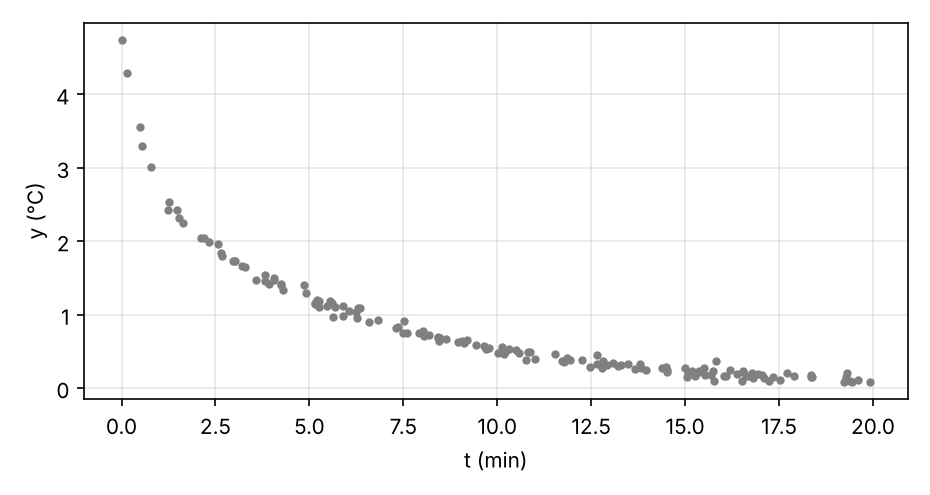
\includegraphics[width=0.62\textwidth]{fig_datos_ejemplo.png}
\caption{Ejemplo de datos (\texttt{datos\_ejemplo.csv}). Los tuyos son distintos pero tienen la misma estructura.}
\end{figure}

\section{Partes del proyecto}

\subsection*{Parte A --- Formulaci\'on (15 pts)}
\begin{enumerate}[label=A\arabic*.]
\item Deduce la jacobiana $\Jm\in\mathbb{R}^{n\times 4}$, $J_{ij}=\partial r_i/\partial\theta_j$, y expresa
$\nabla f=\Jm^\top\rvec$.
\item Escribe la Hessiana exacta $\nabla^2 f=\Jm^\top\Jm+\sum_i r_i\nabla^2 r_i$ y explica cu\'ando es razonable
aproximarla por $\mathbf B=\Jm^\top\Jm$ (Gauss--Newton). ?`Qu\'e propiedad tiene $\mathbf B$ que no tiene la Hessiana
exacta?
\item Verifica tu jacobiana contra diferencias finitas y reporta el error relativo m\'aximo (debe ser
$<10^{-6}$).
\end{enumerate}

\subsection*{Parte B --- Implementaci\'on de los tres minimizadores (35 pts)}
Usa $\gvec=\Jm^\top\rvec$ y $\mathbf B=\Jm^\top\Jm$ en el punto actual $\tht_k$. No est\'a permitido llamar a
\texttt{scipy} dentro de tus implementaciones; \texttt{scipy} se usa \'unicamente para comparar.
\begin{enumerate}[label=B\arabic*.]
\item \textbf{Dogleg (12 pts).} Regi\'on de confianza con modelo $m(\pvec)=\gvec^\top\pvec+\tfrac12\pvec^\top\mathbf B\pvec$:
paso de Cauchy, paso de Gauss--Newton, intersecci\'on de la poligonal con $\norm{\pvec}=\Delta_k$ (ecuaci\'on
cuadr\'atica en $\tau$), raz\'on $\rho_k=\dfrac{f(\tht_k)-f(\tht_k+\pvec_k)}{m(\mathbf 0)-m(\pvec_k)}$, aceptaci\'on si
$\rho_k>0$, y actualizaci\'on de $\Delta_k$ (encoger si $\rho_k<1/4$; crecer si $\rho_k>3/4$ y $\norm{\pvec_k}=\Delta_k$).
\textbf{Tu c\'odigo debe tratar el caso en que $\mathbf B$ es singular o casi singular} y justificar qu\'e paso usa
entonces.
\item \textbf{Levenberg--Marquardt (12 pts).} Resuelve
$\bigl(\mathbf B+\lambda\,\mathrm{diag}(\mathbf B)\bigr)\pvec=-\gvec$, con una regla expl\'icita para $\lambda$ basada en
$\rho_k$ (dec\'ela y \'elala t\'u: reduce $\lambda$ si el paso se acepta, aum\'entalo si se rechaza). Explica por
qu\'e se escala con $\mathrm{diag}(\mathbf B)$ en este problema.
\item \textbf{Gradiente estoc\'astico (11 pts).} Minilotes de tama\~no $m$ (permutaci\'on aleatoria en cada
\'epoca), gradiente del lote $\frac1m\Jm_B^\top\rvec_B$, paso $\alpha_k=\alpha_0/(1+k/k_0)$ y, opcionalmente,
momentum. Debe aceptar \texttt{batch}, \texttt{lr0}, \texttt{k0}, \texttt{epocas} y \texttt{seed}.
\end{enumerate}
Criterios de parada razonables: $\norm{\gvec}_\infty<10^{-6}$ o paso despreciable (Dogleg y LM); n\'umero fijo de
\'epocas (SGD). Documenta los que uses.

\subsection*{Parte C --- Experimentos (30 pts)}
Toma como \emph{soluci\'on de referencia} $\tht^\ast$ la que entrega \texttt{least\_squares(..., method="lm")} con
tolerancias muy peque\~nas (\texttt{xtol=ftol=gtol=1e-15}), y $f^\ast=f(\tht^\ast)$.
\begin{enumerate}[label=C\arabic*.]
\item \textbf{Comparaci\'on (10 pts).} Desde $\tht_0=(1,1,1,0.5)$, completa una tabla con: iteraciones (o pasos),
\emph{evaluaciones de datos}, $f(\tht_{\rm final})$, $\norm{\tht_{\rm final}-\tht^\ast}$ y tiempo, para Dogleg, LM, SGD
y \texttt{least\_squares} (\texttt{lm} y \texttt{trf}). Una \emph{evaluaci\'on de datos} es una fila $(t_i,y_i)$
procesada para calcular residuo y/o jacobiana: en Dogleg/LM cada iteraci\'on cuesta $\approx 2n$ (una pasada en
$\tht_k$ y otra para probar $\tht_k+\pvec_k$); en SGD cada paso cuesta $m$. Grafica $(f-f^\ast)/f^\ast$ en escala
semilogar\'itmica. \textbf{Meta para SGD:} $(f-f^\ast)/f^\ast<5$\,\% (ajusta $\alpha_0$, $k_0$, $m$ o momentum).
\item \textbf{Sensibilidad al punto inicial (10 pts).} Ejecuta Dogleg y LM desde los seis puntos de la
Tabla~\ref{tab:inicios}. Reporta iteraciones y $f$ final en una tabla y dibuja las trayectorias en el plano
$(b,d)$ para al menos tres inicios. Responde: (i) ?`todos los inicios llegan al mismo $f$? (ii) Si alguno no
lo hace, ?`el punto al que llega es un m\'inimo? Justif\'icalo con los autovalores de $\mathbf B$ y de la Hessiana
exacta en ese punto (puedes aproximar esta \'ultima por diferencias finitas de $f$). (iii) ?`Qu\'e pasa con el inicio D y por qu\'e el modelo tiene esa simetr\'ia? (iv) Propone
una forma de eliminar esa ambig\"uedad al reportar $\tht^\ast$.
\item \textbf{Gradiente estoc\'astico (10 pts).} Con $\tht_0=(1,1,1,0.5)$ estudia: tres tama\~nos de lote
(incluye el lote completo $m=n$); paso constante frente a decreciente; momentum (opcional). Una figura con
$(f-f^\ast)/f^\ast$ frente a la \'epoca. Explica con tus datos por qu\'e SGD es mucho m\'as lento que LM en este
problema (relaciona con el n\'umero de condici\'on $\kappa(\Jm^\top\Jm)$) y en qu\'e tipo de problema s\'i ser\'ia la
mejor opci\'on.
\end{enumerate}

\begin{table}[h]
\centering
\caption{Puntos iniciales $\tht_0=(a,b,c,d)$ para C2.}
\label{tab:inicios}
\begin{tabular}{@{}cccccc@{}}
\toprule
A & B & C & D & E & F\\
\midrule
$(1,1,1,0.5)$ & $(5,5,5,5)$ & $(1,0.3,1,0.35)$ & $(1,0.1,1,2)$ & $(3,0.5,0.5,0.05)$ & $(1,1,1,1)$\\
\bottomrule
\end{tabular}
\end{table}

\subsection*{Parte D --- Incertidumbre de los par\'ametros (10 pts)}
En $\tht^\ast$ estima $\hat\sigma^2=2f^\ast/(n-4)$ y la covarianza $\widehat{\mathrm{Cov}}(\tht)=\hat\sigma^2(\Jm^\top\Jm)^{-1}$.
\begin{enumerate}[label=D\arabic*.]
\item Reporta $\tht^\ast$, desviaciones est\'andar e intervalos de confianza de $\approx95$\,\%
($\pm1.98\,\mathrm{sd}$), la matriz de correlaci\'on y $\kappa(\Jm^\top\Jm)$.
\item ?`Qu\'e par\'ametro queda peor determinado y qu\'e par de par\'ametros est\'a m\'as correlacionado? Explica
f\'isicamente (qu\'e informaci\'on aporta la ventana $t\in[0,20]$ sobre cada tasa).
\item Con \texttt{datos\_sinteticos} (en la plantilla) genera datos con tu $\tht^\ast$ y $\sigma\in\{0.05,0.2,0.5\}$,
reajusta con LM y muestra c\'omo cambian las desviaciones est\'andar. ?`Qu\'e relaci\'on observas con $\sigma$?
\end{enumerate}

\subsection*{Parte E --- Informe y c\'odigo (10 pts)}
Informe de m\'aximo 6 p\'aginas (m\'as anexo con c\'odigo si lo deseas) con: formulaci\'on breve, descripci\'on de
cada algoritmo con \emph{tus} decisiones (par\'ametros, reglas, criterios de parada), resultados de C y D con tablas
y figuras legibles, y conclusiones. El archivo \texttt{main.py} debe reproducir todas las tablas y figuras con
\texttt{python main.py datos\_<documento>.csv} y semillas fijas.

\section{R\'ubrica}
\begin{center}
\begin{tabular}{@{}lcp{9.4cm}@{}}
\toprule
\textbf{Parte} & \textbf{Pts} & \textbf{Se eval\'ua}\\
\midrule
A. Formulaci\'on & 15 & jacobiana correcta y verificada; an\'alisis de $\mathbf B$ frente a la Hessiana exacta\\
B. Implementaci\'on & 35 & los tres m\'etodos funcionan y convergen a $\tht^\ast$ (Dogleg y LM) o a la meta (SGD); manejo de $\mathbf B$ singular; reglas de $\rho_k$, $\Delta_k$ y $\lambda$ bien justificadas\\
C. Experimentos & 30 & tablas y figuras correctas; diagn\'ostico del punto estacionario no m\'inimo; an\'alisis de SGD con evidencia\\
D. Incertidumbre & 10 & c\'alculo correcto; interpretaci\'on f\'isica; efecto de $\sigma$\\
E. Informe y c\'odigo & 10 & claridad, reproducibilidad, figuras con ejes y leyendas\\
\midrule
\textbf{Total} & \textbf{100} & \\
\bottomrule
\end{tabular}
\end{center}
\textbf{Bonificaci\'on (m\'ax.\ +10):} (+5) reducir el problema a 2 variables eliminando las amplitudes lineales
$a,c$ por m\'inimos cuadrados lineales en cada evaluaci\'on (\emph{variable projection}) y comparar; (+5) imponer
$b,d>0$ mediante reparametrizaci\'on $b=e^{\beta}$, $d=e^{\delta}$ y comparar.

\section{Referencias sugeridas}
Nocedal \& Wright, \emph{Numerical Optimization}, cap.~4 (regi\'on de confianza, dogleg) y cap.~10 (m\'inimos
cuadrados no lineales, Levenberg--Marquardt); Bottou, Curtis \& Nocedal (2018), \emph{Optimization methods for
large-scale machine learning} (SGD); y el material de las Clases~3 y~4 del curso.
\end{document}
